%=================================================================
% DRAFT MANUSCRIPT -- work in progress, section by section.
% Mirrors the structure/format of futureinternet-4330203-done (1).tex
% (Nouman, Ujjan & Hassanu, MDPI Future Internet), per the same
% supervisor's template, adapted to this project's own dataset,
% methods, and results (see artifacts/paper/tables and thesis_context
% memory for the underlying numbers).
%
% NOTE: Definitions/mdpi.cls is NOT yet present in this repo (the peer
% .tex file references it but the class files weren't included when
% the reference files were added). This document cannot be compiled
% until that class is sourced from MDPI's submission template. Content
% is being drafted in full MDPI-command form now so nothing needs to
% be rewritten once the class is available -- only the \documentclass
% line and packages need the real class file to render.
%=================================================================
\documentclass[futureinternet,article,accept,moreauthors]{Definitions/mdpi}

\firstpage{1}
\makeatletter
\setcounter{page}{\@firstpage}
\makeatother
\pubvolume{1}
\issuenum{1}
\articlenumber{0}
\pubyear{2026}
\copyrightyear{2026}
\externaleditor{Firstname Lastname}
\datereceived{ }
\daterevised{ }
\dateaccepted{ }
\datepublished{ }
\hreflink{https://doi.org/}

\usepackage[utf8]{inputenc}
\usepackage{graphicx}
\usepackage{float}
\usepackage{tabularx}
\usepackage{changepage}
\usepackage{array}
\usepackage{ragged2e}
\usepackage[T1]{fontenc}
\usepackage{booktabs}

%=================================================================
% TITLE -- DRAFT, needs confirmation. Mirrors the peer paper's
% "[qualifier] Anomaly Detection for [traffic] Using [method A] with
% [method B]" pattern.
\Title{Content- and Session-Aware Anomaly Detection for Web Server Logs Using a Fused Autoencoder and Variational LSTM Framework: A Cross-Dataset Evaluation}

% AUTHOR BLOCK -- DRAFT. Matches the peer paper's author-role pattern
% (student first/corresponding author, supervisor + moderator as
% co-authors). NOTE: the moderator's name is spelled inconsistently
% across source documents ("Muhsin Husseinu" on the thesis title page,
% "Muhsin Hussenu" in the thesis body/acknowledgements, "Muhsin
% Hassanu" in the peer paper) -- needs to be confirmed with the
% moderator directly before submission, not guessed.
\Author{Abdul Rehman *, Raja Ujjan and Muhsin Hussenu *}

\AuthorNames{Abdul Rehman, Raja Ujjan, and Muhsin Hussenu}

\address[1]{Department of Computing and Cybersecurity, University of the West of Scotland, London Campus, London E14 2BA, UK}

\corres{Correspondence: [student email TBD] (A.R.)}

\abstract{%TODO: write after Results/Discussion are finalized, so the
reported numbers are locked. Draft note: should mirror the peer
paper's abstract shape -- motivation, gap, framework summary,
datasets, headline quantitative results, one-sentence takeaway.
Numbers to pull from once ready: artifacts/paper/tables/ablation_table.csv,
fusion_sweep.csv, threshold_transfer.csv, baseline_comparison.csv,
latency_benchmark.json, session_v1_vs_v2.csv (source of truth --
not the original thesis Table 5.6 figures, several of which this
re-run diverges from).}

\keyword{web server logs; anomaly detection; autoencoder; variational LSTM; session modelling; score fusion; cross-dataset generalisation}

\begin{document}

\section{Introduction}

Web applications underpin most critical digital services in use today, from banking and healthcare to e-commerce and cloud infrastructure, and their continuous, public-facing exposure makes them a persistent target for attackers~\cite{scarfone2007}. Every request a web server processes is recorded in an access log, together with metadata such as the request method, path, response status, and client identifiers. These logs are one of the richest available sources of security-relevant information: in principle, they capture both the legitimate use of an application and the traces left by attackers probing or exploiting it. In practice, however, the volume and variety of this data make manual inspection infeasible for any application of meaningful scale, and organisations have long relied on signature-based intrusion detection and rule-based filtering to triage it~\cite{scarfone2007}.

Signature- and rule-based approaches are effective against known attack patterns but are structurally unable to detect zero-day or previously unseen attacks, since they can only recognise what has already been catalogued. This has motivated a shift towards anomaly detection, which instead models what \emph{normal} traffic looks like and flags deviations from it, without requiring the deviation to match a predefined signature~\cite{chandola2009}. Anomaly detection is a natural fit for web security because it does not depend on a labelled corpus of known attacks -- which is difficult to obtain, quickly goes stale, and can never be assumed complete -- but it introduces its own difficulties. Web traffic is highly non-stationary: normal behaviour drifts as applications change, and it can vary enormously between different endpoints, user populations, and even times of day. Attack traffic is also typically a tiny fraction of the total volume, so any evaluation of an anomaly detector must be designed around severe class imbalance rather than raw accuracy~\cite{chandola2009}.

Deep learning has extended anomaly detection to log and web-traffic data by learning representations directly from raw or lightly processed records, rather than requiring hand-engineered features. Sequence models such as LSTMs have been used to learn the normal structure of a stream of log events and flag deviations from it~\cite{nedelkoski2020}, and DeepLog demonstrated that treating a system log as a natural-language-like sequence allows an LSTM to learn normal execution patterns and detect anomalies as departures from them~\cite{du2017}. Applied to HTTP traffic specifically, this behavioural, sequence-oriented view is complementary to a second, request-level view: individual HTTP requests can themselves be modelled directly, using an autoencoder trained to reconstruct the structural and payload characteristics of normal requests, so that unusually large reconstruction error flags anomalous content such as injection payloads or malformed parameters. Recent work combining a variational LSTM autoencoder with a deviation network for exactly this purpose has shown that this class of model is well suited to detecting web attacks directly from HTTP weblogs~\cite{jagat2024}.

These two views, however, are not interchangeable. A content-based model that scores individual requests in isolation cannot see attacks that only become apparent across a sequence of otherwise unremarkable requests -- reconnaissance-style scanning, credential stuffing, or low-and-slow probing, for example, where each individual request may be syntactically valid. A behaviour-based model that scores sequences of requests grouped by client can catch exactly this class of attack, but it depends on there being a genuine sequence to model in the first place: if a client only issues one or two requests, or if requests from a given client cannot be reliably grouped together, there is no behavioural signal to learn from. This dependency on session structure is not merely a theoretical caveat -- as this study's own experiments later show (Section~\ref{sec5}), it materially determines whether a session-based branch can contribute anything at all for a given traffic sample.

Because content-based and behaviour-based detectors fail in different, largely non-overlapping ways, combining their outputs is a natural way to cover more of the attack surface than either can alone. Hybrid, fusion-based frameworks that integrate multiple detection signals have been shown to improve robustness and stability relative to single-model detectors, particularly under the kind of severe class imbalance and limited labelled data that characterises real security settings~\cite{kamal2025}. Realising this benefit in practice, however, depends heavily on how the resulting system is evaluated. A large share of the anomaly-detection literature reports results on a single dataset, which risks overstating how well a method will generalise once deployed against traffic with different structure, format, or attack composition than whatever it was tuned against. This concern is well established in the wider intrusion-detection literature, where the design of benchmark datasets themselves -- their realism, diversity, and reproducibility -- has long been recognised as a determining factor in whether reported results are meaningful outside the dataset they were produced on~\cite{shiravi2012}.

Despite the individual maturity of content-based autoencoders, behaviour-based sequence models, and fusion-based detection frameworks, their combined application to web server logs specifically, evaluated across genuinely different log formats and under a strict cross-dataset protocol -- where a detection threshold is fixed on one data source and applied unchanged to others, rather than recalibrated on each dataset in turn -- remains underexplored. Many studies that do combine content and behavioural signals validate the result on a single log format and a single traffic sample, leaving open how such a system behaves when the underlying session structure, log schema, or class balance of the target traffic differs substantially from what the model was built on.

To address this gap, this work presents a hybrid anomaly detection framework for web server logs that combines a content-based autoencoder, trained to reconstruct the structural features of individual HTTP requests, with a session-based variational LSTM autoencoder, trained on genuine per-client request sequences rather than an arbitrary sliding window over the raw log stream. The outputs of the two branches are combined through score-level fusion, and the resulting framework is evaluated not only within a single dataset but across three structurally different sources: two self-generated Apache-style access-log corpora and a structured Nginx JSON log, together with the publicly available CSIC~2010 HTTP dataset, which additionally serves as the source domain for a cross-dataset threshold-transfer evaluation in which a single fixed decision threshold, calibrated once on genuinely benign traffic, is applied unchanged to unseen target datasets.

The remainder of this paper is organised as follows. Section~\ref{sec2} sets out the specific contributions of this work. Section~\ref{sec3} reviews related work on anomaly detection for web and log data, content- and behaviour-based deep learning models, and hybrid/fusion-based detection frameworks. Section~\ref{sec4} describes the datasets, preprocessing, feature representation, model architectures, and evaluation protocol. Section~\ref{sec5} presents the experimental results, including the branch ablation, fusion-weight sensitivity, classical-baseline comparison, and cross-dataset threshold-transfer experiments. Section~\ref{sec6} discusses these findings and their practical implications, and Section~\ref{sec7} concludes the paper and outlines directions for future work.

\section{Research Contributions} \label{sec2}

This paper makes the following contributions.

First, we build a hybrid system that finds anomalies in web server logs using two parts. One part checks each request on its own, using an autoencoder. The other part checks a sequence of requests from the same client, using a variational LSTM. We combine the two scores into one final score, so the system can catch both strange single requests and strange patterns of behaviour over time.

Second, we find and fix a real problem in how the behaviour part was trained. In the old version, the model was trained using a plain sliding window over the whole log. This window did not check which client sent each request, so requests from different clients could end up mixed in the same window. We fix this by grouping requests by client (IP address and user agent) first, so each window only holds requests from one real client. This fix makes a big difference: on the CSIC~2010 dataset, where one client sends many requests in a row, the behaviour part's AUC score rises from about 0.63 to about 0.97 after the fix.

Third, this work reports an honest and useful finding about the data itself. Some of our datasets have only one request per client. In real per-session detection, if a client only sends one request, there is no sequence to check, so the behaviour part gives no score at all for that data. We treat this as a fact about the data, not a failure of the method, and we explain it clearly instead of hiding it. This shows that a true session-based model only helps when the traffic actually has multi-request sessions in it.

Fourth, we test the system on more than one kind of log. We use two Apache-style logs we built ourselves, one Nginx JSON log, and the public CSIC~2010 HTTP dataset. Testing across different log formats and different datasets shows whether the method still works when the data changes shape.

Fifth, we run a cross-dataset test that checks if a threshold set on one dataset still works on another. We set the detection threshold using only the CSIC data, and only its normal, non-attack traffic. Then we use that same threshold, with no change, on three other datasets. The result is surprising: F1 score goes up, not down, when we use the frozen CSIC threshold instead of a threshold tuned on each dataset on its own. For example, on the Access Eval Mix 2000 dataset, the fused F1 score rises from about 0.12 (tuned on that dataset) to about 0.67 (using the frozen CSIC threshold). This happens because these test datasets contain a lot of attack traffic, so a threshold tuned only on them is not a fair "normal traffic" threshold. This is a useful, real finding about how to set thresholds in practice.

Sixth, we compare our system with simple baseline methods: Random Forest, which uses attack labels during training, and Isolation Forest and One-Class SVM, which do not use labels, like our own method. We also measure how fast the system runs. On average, scoring one request takes about 0.14~ms for the content part and about 0.08~ms for the behaviour part when done one request at a time, and scoring in batches is much faster, at about 630{,}000 lines per second. This shows the system could run in near real time.

Together, these results show that a two-part fusion system can work well across different kinds of web log data, and that fixing how sessions are built and how thresholds are set can matter as much as the choice of model itself.

\section{Related Work} \label{sec3}

\subsection{Anomaly Detection in Web Server Logs}

Web server logs record every request a server handles. Each line usually has the request method, the URL, the response code, the time, and the client's IP address. Security teams can use these logs to find attacks, but there are far too many lines to check by hand. For a long time, most systems used rules or signatures to spot bad requests~\cite{scarfone2007}. Rules like this work well for known attacks, but they cannot catch new or changed attacks, because they only look for patterns someone has already written down. This is why anomaly detection is useful: instead of matching known attack patterns, it learns what normal traffic looks like and flags anything that looks different~\cite{chandola2009}. This can catch attacks that have never been seen before, but it is harder to build well, because normal web traffic changes over time and attacks are a very small part of all traffic.

\subsection{Classical Machine Learning Methods}

Before deep learning became common, many studies used classic machine learning methods for this problem. Isolation Forest is one of the most used. It works by randomly splitting the data again and again; points that get cut off quickly, after only a few splits, are treated as anomalies~\cite{liu2008}. This method does not need labelled attack data, runs fast, and is simple to set up, which is why it is still used today. For example, one recent study applied Isolation Forest directly to web traffic logs from an e-commerce site and showed it can tell normal and anomalous requests apart without needing attack labels~\cite{chua2024}. Other classic methods, such as clustering and one-class classifiers, have also been used, but they often need features to be picked and built by hand, and they can struggle when the traffic pattern changes.

\subsection{Content-Based Deep Learning}

Deep learning removes the need for hand-built features by learning directly from the raw or lightly processed request data. One common approach is the autoencoder. An autoencoder learns to compress a normal request into a small representation and then rebuild it. If the model is trained only on normal requests, it becomes good at rebuilding normal requests but bad at rebuilding attack requests, so a request with a high rebuild error can be flagged as an anomaly. One study used this idea end to end, training a deep autoencoder directly on HTTP requests, and showed it could detect attacks such as SQL injection and cross-site scripting without needing much labelled data~\cite{pan2019}. Models like this are good at finding strange or broken single requests, but they look at each request on its own, so they cannot see attacks that only show up across many requests over time.

\subsection{Behaviour-Based Deep Learning}

To catch attacks that unfold over several requests, other work models the order and pattern of requests instead of looking at single requests. LSTM networks are built for this, since they can learn from a sequence of past events. DeepLog treats a stream of log lines like a sentence, learning the normal order of events and flagging any sequence that breaks the learned pattern~\cite{du2017}. Later work used a self-attention model, instead of or alongside an LSTM, to learn which parts of a log sequence matter most for telling normal and abnormal apart~\cite{nedelkoski2020}. Closer to our own work, one study built a variational LSTM autoencoder combined with a deviation network, trained directly on HTTP weblogs, and showed it can detect web attacks by modelling normal session behaviour~\cite{jagat2024}. Behaviour-based models like these can catch attacks that content-based models miss, such as scanning or repeated probing, but they need enough real, connected requests from the same client to learn from. If a client only sends one or two requests, there is no real sequence to learn from -- a point this paper returns to directly in Section~\ref{sec5}.

\subsection{Hybrid and Fusion-Based Detection}

Since content-based and behaviour-based models catch different kinds of attacks, several studies combine both into one system. The idea is to score each request or session with more than one model, then merge the scores into a single final decision. This kind of hybrid, fusion-based design has been shown to work better than either model alone, especially when labelled attack data is scarce and normal traffic looks very different from attack traffic~\cite{kamal2025}. Building a good fusion system is not simple, though: the two branches usually need to be trained and set up carefully so that one does not drown out the other, and the merged score still needs its own threshold.

\subsection{Cross-Dataset Evaluation}

Most of the studies above are tested on a single dataset. This is a real problem, because a model that works well on the data it was tuned on may not work as well on new data with a different shape, format, or mix of attacks. Building good benchmark datasets for intrusion detection, and testing across more than one of them, has long been seen as important for getting results that mean something outside the exact dataset used~\cite{shiravi2012}. A recent study looked at this problem directly for network intrusion detection: models that scored close to perfect when trained and tested on the same dataset dropped close to random guessing when tested on a different dataset, showing how easy it is to overstate a model's real performance with single-dataset testing~\cite{cantone2024}. This is the exact gap this paper addresses for web server logs: testing across more than one log format, and running a true cross-dataset threshold test, where the decision threshold is set once and never changed for new data.

\subsection{Summary}

Table~\ref{tab:lit_review} lists the studies discussed above, the kind of method each one uses, the kind of data it was tested on, and the main gap that this paper tries to close.

\begin{table}[H]
\caption{Summary of related studies on web and log anomaly detection.}
\label{tab:lit_review}
\scriptsize
\begin{adjustwidth}{-\extralength}{0cm}
\begin{tabularx}{\fulllength}{l l l l m{4.5cm}<{\raggedright}}
\toprule
\textbf{Study} & \textbf{Method} & \textbf{Data Type} & \textbf{Evaluation} & \textbf{Main Limitation} \\
\midrule

Scarfone and Mell~(2007)~\cite{scarfone2007} & Rule-based IDS/IPS guidance & Network traffic & Guidance document & Rules only catch known attack patterns \\

Chandola et al.~(2009)~\cite{chandola2009} & Survey & General & Review study & No single detector proposed \\

Liu et al.~(2008)~\cite{liu2008} & Isolation Forest & General tabular data & Benchmark datasets & Not evaluated on web request logs \\

Chua et al.~(2024)~\cite{chua2024} & Isolation Forest & Web traffic logs & Single dataset & Single detection view, no behaviour model \\

Pan et al.~(2019)~\cite{pan2019} & Stacked denoising autoencoder & HTTP requests & Single dataset & Scores single requests only, no session view \\

Du et al.~(2017)~\cite{du2017} & LSTM (DeepLog) & System logs & Single dataset & Not web-request specific \\

Nedelkoski et al.~(2020)~\cite{nedelkoski2020} & Self-attention classifier & Unstructured logs & Single dataset & No cross-dataset test reported \\

Jagat et al.~(2024)~\cite{jagat2024} & Variational LSTM autoencoder + deviation network & HTTP weblogs & Single dataset & No content-based branch, single dataset \\

Kamal and Mashaly~(2025)~\cite{kamal2025} & Hybrid deep learning IDS & Network traffic & Single dataset & Single dataset, not web-log specific \\

Shiravi et al.~(2012)~\cite{shiravi2012} & Benchmark dataset design & Network traffic & Dataset study & Dataset paper, no detection model \\

Cantone et al.~(2024)~\cite{cantone2024} & Multiple classical ML models & Network traffic & Cross-dataset & Not applied to web-log or hybrid deep models \\

\bottomrule
\end{tabularx}
\end{adjustwidth}
\end{table}
\unskip

\section{Materials and Methods} \label{sec4}

\subsection{Research Design Overview}

This study follows an experimental design. We build and train the models directly on real log data, then test them and report what we find. The setup is semi-supervised: both models are trained only on requests known to be normal, so no attack labels are needed to build the models themselves. Attack labels are only used afterwards, to check how well each trained model tells normal and attack traffic apart. The full process has five steps: preparing the data, building request-level and session-level features, training the two branch models, combining their scores through fusion, and setting a decision threshold. Each step is described below.

\subsection{Datasets} \label{sec4.2}

We use eight datasets in total, listed in Table~\ref{tab:datasets}. One of them, the CSIC~2010 HTTP dataset, is a public dataset built by the Information Security Institute of CSIC (the Spanish National Research Council), for testing web attack detection on an e-commerce application~\cite{csic2010}. It has 61{,}065 requests in total: 36{,}000 normal and 25{,}065 attack requests. It is the only dataset in this study that is not self-generated.

The rest of the datasets were generated for this project's own testbed, using normal browsing traffic mixed with known attack tools (such as sqlmap and nikto) run against a small test web application, following an approach also used elsewhere in the intrusion-detection literature for building test data~\cite{shiravi2012}. Three of these self-generated logs are used as target datasets for the cross-dataset test described in Section~\ref{sec4.7}: Access Eval Mix 2000, Access Eval Small 500, and Nginx JSON Eval 800, which is the only one of the three stored as structured JSON lines rather than a plain Apache-style text log. The remaining four datasets support the branch ablation study, the classical-baseline comparison, and the training of the session model: Access Attacks 200, Access Mixed 500, Access Small Benign, and Access Super Long Session 2000, which is entirely normal traffic from a single client sending a long run of requests, used only to help train the session model.

An important detail, revisited in Section~\ref{sec5}, is that most of the self-generated logs are attack-heavy rather than normal-heavy. For example, 81\% of Access Eval Mix 2000 is attack traffic. This matters because a threshold set directly on one of these datasets is not really a "normal traffic" threshold, since most of what it sees is not normal.

\begin{table}[H]
\caption{Datasets used in this study.}
\label{tab:datasets}
\begin{tabularx}{\textwidth}{lXCCCl}
\toprule
\textbf{Dataset} & \textbf{Format} & \textbf{Total} & \textbf{Normal} & \textbf{Attack} & \textbf{Role} \\
\midrule
CSIC 2010 & Public, e-commerce app & 61{,}065 & 36{,}000 & 25{,}065 & Source domain; session training \\
Access Eval Mix 2000 & Apache Combined & 2{,}000 & 380 & 1{,}620 & Target dataset \\
Access Eval Small 500 & Apache Combined & 500 & 107 & 393 & Target dataset \\
Nginx JSON Eval 800 & Structured JSON & 800 & 174 & 626 & Target dataset \\
Access Attacks 200 & Apache Combined & 200 & 36 & 164 & Ablation, baselines \\
Access Mixed 500 & Apache Combined & 500 & 205 & 295 & Ablation, baselines \\
Access Small Benign & Apache Combined & 120 & 54 & 66 & Ablation, baselines \\
Access Super Long Session 2000 & Apache Combined & 2{,}000 & 2{,}000 & 0 & Session training only \\
\bottomrule
\end{tabularx}
\end{table}

\subsection{Data Preprocessing and Feature Extraction}

Each log line is first parsed into a common set of fields: client IP address, timestamp, request method, path, response status, response size, and, where available, the user agent string. Three log line formats are supported: Apache Combined (which includes referrer and user agent), Apache Common (without those two fields), and structured JSON lines, so that Nginx JSON Eval 800 can be parsed with the same pipeline as the Apache-style logs.

From each parsed line, we build one feature vector with 11 numbers, listed in Table~\ref{tab:features}. This is a light, structural view of a request: it looks at the shape of the request and the server's response to it, not at the request body or query values directly. The same 11 numbers are used for both branches; the only difference is that the session branch groups these vectors into short sequences (Section~\ref{sec4.5}), while the content branch scores one vector at a time.

Before training, feature values are scaled with a standard scaler (zero mean, unit variance), fitted separately for the content model and the session model, using only the data each model is trained on.

\begin{table}[H]
\caption{The 11 features built from each parsed request.}
\label{tab:features}
\begin{tabularx}{\textwidth}{lX}
\toprule
\textbf{Feature} & \textbf{Meaning} \\
\midrule
Method code & HTTP method mapped to a small integer (e.g., GET = 1, POST = 2) \\
Path length & Number of characters in the request path \\
Is API & 1 if the path starts with \texttt{/api/}, else 0 \\
Has query & 1 if the path has a query string, else 0 \\
Has file extension & 1 if the path looks like a file (has a dot before any query string), else 0 \\
Status code & Raw HTTP response status code \\
Status 2xx / 3xx / 4xx / 5xx & Four yes/no flags for which hundred-range the status code falls in \\
Log response size & Natural log of the response size in bytes \\
\bottomrule
\end{tabularx}
\end{table}

\subsection{Content-Based Autoencoder}

The content branch is a small feed-forward autoencoder. The encoder has four layers that shrink the 11 input numbers down to a 4-number summary ($11 \rightarrow 32 \rightarrow 16 \rightarrow 8 \rightarrow 4$), each followed by a ReLU activation. The decoder mirrors this, growing the summary back up to 11 numbers ($4 \rightarrow 8 \rightarrow 16 \rightarrow 32 \rightarrow 11$), with no activation on the last layer, since its output needs to match the original values directly.

The model is trained only on requests known to be normal, using the mean squared error between the input and its rebuilt version as the loss, optimised with Adam (learning rate 0.001). At test time, the same mean squared error is used as the anomaly score for each request: a normal-looking request should be rebuilt closely, so a high error suggests the request does not look like anything the model saw as normal.

\subsection{Session-Based Variational LSTM Autoencoder} \label{sec4.5}

The session branch models short sequences of requests from the same client, rather than single requests on their own. A client is identified by the pair (IP address, user agent).

In the original thesis code, session windows were built by sliding a fixed-size window over the whole log in time order, without checking which client sent each request. A single window could therefore mix requests from several different clients. We treat this as a real bug, not a design choice, and fix it in this study: windows are now built only from the requests belonging to one client at a time, so a window of length 20 always holds 20 requests from a single real client, never a mix.

The model is a variational autoencoder built from two LSTM networks. An LSTM encoder reads a window of requests and produces a mean and a variance for a small latent space (size~8). A latent value is drawn from this distribution only during training; at test time, the mean is used directly, so scoring is repeatable rather than random. A second LSTM decoder then rebuilds the whole window from this one latent value, repeated at every step. The training loss adds the mean squared reconstruction error to a KL-divergence term that keeps the latent space close to a standard normal distribution, with the KL term weighted at 0.001. As with the content branch, training uses only normal traffic and the Adam optimiser (learning rate 0.001).

Building real per-client windows needs enough requests from the same client, so the session model is trained on normal traffic pooled from two sources: the normal-labelled requests in CSIC~2010 (36{,}000 requests, almost all from the same two clients) and the fully normal Access Super Long Session 2000 log (2{,}000 requests from a single client). Together these give 38{,}000 requests, which build into 7{,}594 real per-client session windows of length 20, using a stride of 5 requests between windows.

At test time, scoring also uses a real rolling buffer, one client at a time: the first 19 requests from a client fill the buffer, and a session score is only produced once 20 requests from that same client have arrived. This matches how windows are built during training. We call this the corrected session model for the rest of this paper, and compare it directly against the original, uncorrected version in Section~\ref{sec5}.

\subsection{Fusion and Anomaly Scoring}

Once both branches produce a score for a request, the two scores are combined into one fused score by a weighted average:
\begin{equation}
s_{\text{fused}} = \frac{w_c \cdot s_c + w_s \cdot s_s}{w_c + w_s}
\end{equation}
where $s_c$ and $s_s$ are the content and session scores and $w_c$, $w_s$ are their weights. The content branch always scores every request; the session branch only scores a request once its client's buffer is full, so early requests from a new client are scored on content alone. If only one branch has a score for a given request, the fused score is simply that branch's score. The default weights are $w_c = w_s = 0.5$; Section~\ref{sec5} reports what happens when this balance is changed.

\subsection{Threshold Selection and Cross-Dataset Transfer} \label{sec4.7}

A request is flagged as anomalous when its score is above a threshold. Following the approach used in the original thesis work, thresholds are set as a percentile of the score distribution, with the 95th percentile as the default, so only the highest-scoring 5\% of requests are flagged.

Two ways of setting this threshold are compared in this paper. \textbf{Self-calibrated thresholding} sets the percentile threshold directly on the dataset being tested, using every request in it, normal and attack alike. This is what the original thesis work did. \textbf{Cross-dataset threshold transfer} instead sets the threshold once, using only the normal-labelled requests from CSIC~2010, and then applies that one fixed threshold, unchanged, to the three target datasets, without ever looking at their own scores. This second approach is closer to how a real detector would be used: a threshold is set once, using traffic known to be normal, and then applied to new data it has never seen. Section~\ref{sec5} compares the two directly.

\subsection{Evaluation Metrics}

Because attack traffic is a small share of the total in most anomaly detection settings, and a large share in some of the self-generated datasets used here, accuracy on its own is not a useful measure. We report the area under the ROC curve (AUC) and the area under the precision-recall curve (PR-AUC), which do not depend on a single threshold, together with threshold-dependent measures: precision, recall, F1 score, and false positive rate (FPR), plus the full confusion matrix.

\subsection{Implementation and Reproducibility}

All models are implemented in Python, using PyTorch for the autoencoder and the variational LSTM autoencoder, and scikit-learn for scaling, classical baselines, and metric calculations. Both models are trained with a fixed random seed, so repeated training runs give the same result. Trained models, scalers, and score outputs for every dataset are saved to disk, so results can be reproduced without retraining.

\section{Results} \label{sec5}

\subsection{Effect of the Session Construction Fix}

Table~\ref{tab:session_fix} compares the original (uncorrected) session model against the corrected model described in Section~\ref{sec4.5}, on the two datasets that have any real per-client session structure to score: CSIC~2010, where almost all requests come from the same two clients, and Access Super Long Session 2000, a single client sending 2{,}000 requests in a row with no attack traffic at all, so no threshold-based score is meaningful there.

On CSIC~2010, the fix makes a large difference. The session branch's AUC rises from 0.63 with the original model to 0.97 with the corrected model, and its F1 score rises from 0.14 to 0.22, with precision reaching 1.00.

On the other six datasets (Access Eval Mix 2000, Access Eval Small 500, Nginx JSON Eval 800, Access Attacks 200, Access Mixed 500, Access Small Benign), the corrected model produces no session score at all, because, as Table~\ref{tab:datasets} already suggests, almost every request in these logs comes from a different client. A true per-client model needs at least 20 requests from the same client before it can score anything, and these logs never reach that. This is not a weakness of the fix; it is a fact about the data. The original, uncorrected model scored every single line in these logs, but it did so by mixing unrelated clients into the same window, so that full coverage was not a real strength.

\begin{table}[H]
\caption{Session branch, before and after the session construction fix.}
\label{tab:session_fix}
\begin{tabularx}{\textwidth}{lCCCCC}
\toprule
\textbf{Dataset} & \textbf{Model} & \textbf{Requests Scored} & \textbf{AUC} & \textbf{F1} & \textbf{Precision} \\
\midrule
CSIC 2010 & Original & 61{,}065 & 0.63 & 0.14 & 0.64 \\
CSIC 2010 & Corrected & 61{,}065 & 0.97 & 0.22 & 1.00 \\
Access Eval Mix 2000, and 5 others & Original & all lines & 0.55--0.67 & 0.09--0.16 & 0.78--1.00 \\
Access Eval Mix 2000, and 5 others & Corrected & 0 & --- & --- & --- \\
\bottomrule
\end{tabularx}
\end{table}

\subsection{Branch Ablation}

Table~\ref{tab:ablation} reports AUC and F1 for the content, session, and fused branches on every dataset, using the corrected session model throughout. Figure~\ref{fig:heatmap_auc} shows the same AUC values as a heatmap, making it easier to see where each branch does well.

The content branch reaches a moderate AUC (roughly 0.60--0.70) on most datasets, with high or perfect precision but low recall (roughly 0.06--0.09), because the 95th-percentile threshold only flags the most extreme-looking requests. This matches the precision-first design already used in the original thesis work: fewer, more trustworthy alerts over broad coverage.

The session branch only produces a score on CSIC~2010, for the reason given above. On that dataset it clearly beats the content branch (AUC 0.97 vs. 0.70).

The fused branch, on CSIC~2010, sits between the two single branches (AUC 0.77), better than content alone but worse than session alone. On the six datasets without a session score, the fused branch is identical to the content branch, since there is nothing to fuse with. Access Super Long Session 2000 is entirely normal traffic, so its AUC cannot be computed at all (there is only one class), and its F1 is 0 for every branch.

\begin{table}[H]
\caption{Branch ablation: AUC and F1 by dataset, using the corrected session model.}
\label{tab:ablation}
\begin{adjustwidth}{-\extralength}{0cm}
\begin{tabularx}{\fulllength}{lCCCCCC}
\toprule
\textbf{Dataset} & \textbf{Content AUC} & \textbf{Session AUC} & \textbf{Fused AUC} & \textbf{Content F1} & \textbf{Session F1} & \textbf{Fused F1} \\
\midrule
CSIC 2010 & 0.70 & 0.97 & 0.77 & 0.14 & 0.22 & 0.14 \\
Access Eval Mix 2000 & 0.69 & --- & 0.69 & 0.12 & --- & 0.12 \\
Access Eval Small 500 & 0.70 & --- & 0.70 & 0.12 & --- & 0.12 \\
Nginx JSON Eval 800 & 0.66 & --- & 0.66 & 0.11 & --- & 0.11 \\
Access Attacks 200 & 0.47 & --- & 0.47 & 0.11 & --- & 0.11 \\
Access Mixed 500 & 0.60 & --- & 0.60 & 0.16 & --- & 0.16 \\
Access Small Benign & 0.63 & --- & 0.63 & 0.17 & --- & 0.17 \\
Access Super Long Session 2000 & n/a & n/a & n/a & 0.00 & 0.00 & 0.00 \\
\bottomrule
\end{tabularx}
\end{adjustwidth}
\end{table}
\unskip

\begin{figure}[H]
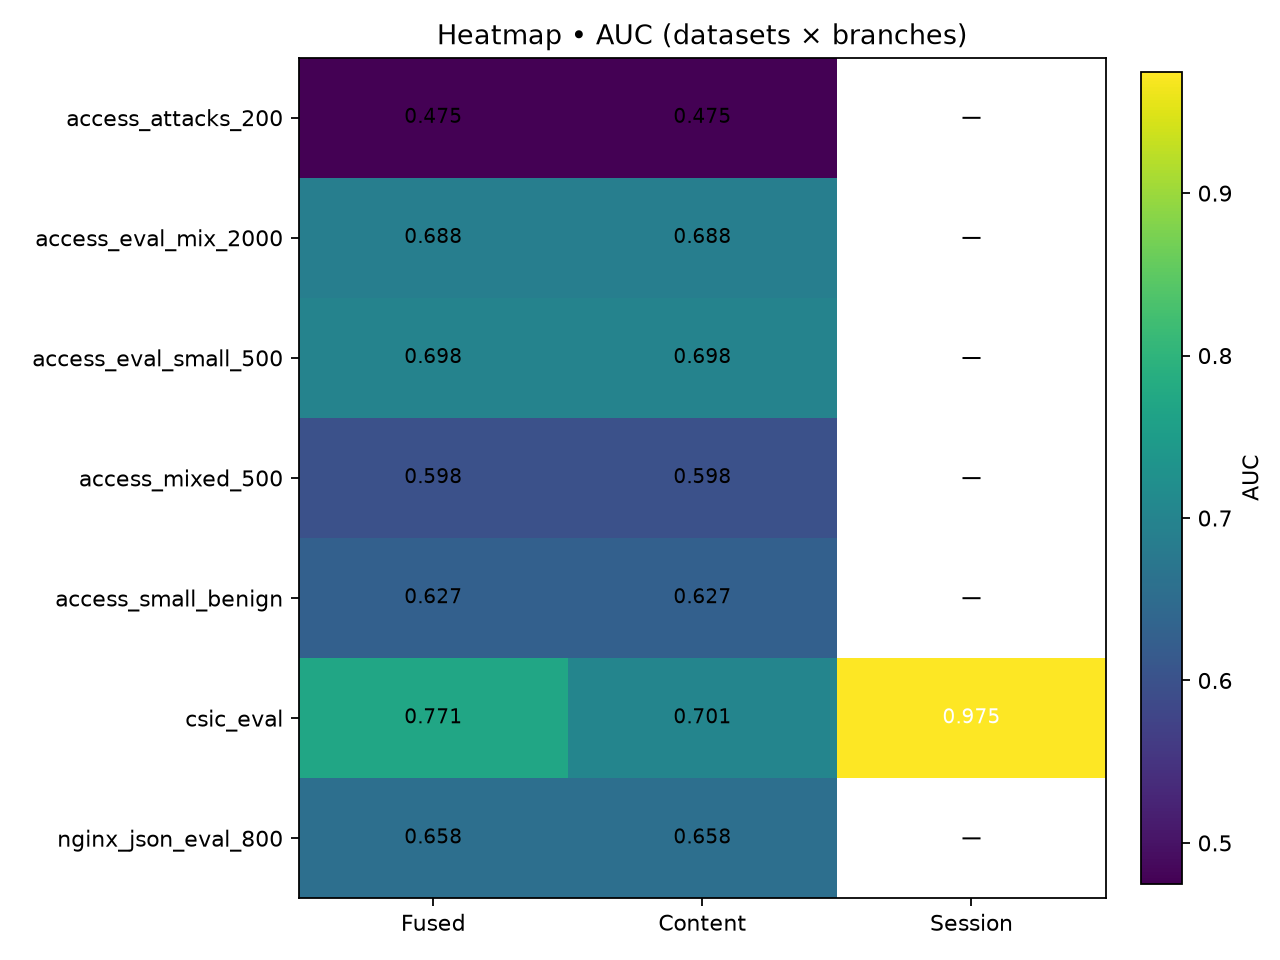
\includegraphics[width=0.72\textwidth]{../artifacts/paper/figures/heatmap_auc.png}
\caption{AUC by dataset and branch (content, session, fused).}
\label{fig:heatmap_auc}
\end{figure}

\subsection{Fusion Weight Sensitivity}

Because a session score only exists for CSIC~2010, this is the only dataset where changing the fusion weight has any effect. Table~\ref{tab:fusion_sweep} sweeps the weight given to each branch, from content-only ($w_c=1$) to session-only ($w_s=1$).

AUC and F1 both rise steadily as more weight is put on the session branch, and the best score on both measures is reached at full session weight, not at any blended point in between. This means that, for this dataset, mixing in the content branch never helps; it only pulls the fused score away from the stronger session branch. This goes against the usual assumption that fusing two branches is always better than picking the stronger one, and it is worth stating plainly rather than glossing over. On the other seven datasets, sweeping the weight has no effect, since only a content score exists there.

\begin{table}[H]
\caption{Fusion weight sweep on CSIC 2010.}
\label{tab:fusion_sweep}
\begin{tabularx}{\textwidth}{CCCC}
\toprule
\boldmath{$w_c$} & \boldmath{$w_s$} & \textbf{AUC} & \textbf{F1} \\
\midrule
1.0 & 0.0 & 0.70 & 0.14 \\
0.7 & 0.3 & 0.75 & 0.14 \\
0.5 & 0.5 & 0.77 & 0.14 \\
0.3 & 0.7 & 0.78 & 0.15 \\
0.0 & 1.0 & \textbf{0.97} & \textbf{0.22} \\
\bottomrule
\end{tabularx}
\end{table}

\subsection{Cross-Dataset Threshold Transfer}

Table~\ref{tab:threshold_transfer} compares the two ways of setting the decision threshold described in Section~\ref{sec4.7}: self-calibrated (tuned separately on each target dataset, using every row in it) and transferred (set once on CSIC~2010's normal traffic only, then applied unchanged). AUC does not change between the two, since AUC does not depend on a threshold; only precision, recall, F1, and false positive rate change.

The result is the opposite of what we expected going in. Using the transferred threshold raises F1 on every target dataset, not by a small amount, but by roughly four to five times. For example, on Access Eval Mix 2000, the fused branch's F1 rises from 0.12 (self-calibrated) to 0.67 (transferred). The same pattern holds on Access Eval Small 500 (0.12 to 0.67) and Nginx JSON Eval 800 (0.11 to 0.67), and for the content branch alone on all three datasets.

The reason is the point already raised in Section~\ref{sec4.2}: these three target datasets are attack-heavy, not normal-heavy (81\%, 79\%, and 78\% attack traffic, respectively). A threshold set at the 95th percentile of a dataset that is mostly attack traffic ends up far too high, since it is really the 95th percentile of a mostly-attack distribution, not a normal-traffic distribution, so it only catches the most extreme 5\% of an already unusual mix. The frozen CSIC threshold, by contrast, is set on genuinely normal traffic, so it sits at a more sensible point and catches far more real attacks, at the cost of a higher false positive rate (up to about 0.30--0.36 on the fused branch, compared to 0.00--0.02 self-calibrated).

This is a useful, practical finding: on these datasets, what data a threshold is calibrated on matters more than whether it is calibrated on the same dataset being tested. A threshold set on real normal traffic, even from a completely different dataset, can work better than one set on the target dataset itself, if that target dataset does not actually represent normal conditions well.

\begin{table}[H]
\caption{Self-calibrated vs. transferred threshold, on the three target datasets.}
\label{tab:threshold_transfer}
\begin{adjustwidth}{-\extralength}{0cm}
\begin{tabularx}{\fulllength}{llCCCCCC}
\toprule
\textbf{Target Dataset} & \textbf{Branch} & \textbf{AUC} & \textbf{Self F1} & \textbf{Self FPR} & \textbf{Transf. F1} & \textbf{Transf. Recall} & \textbf{Transf. FPR} \\
\midrule
Access Eval Mix 2000 & Content & 0.69 & 0.12 & 0.00 & 0.54 & 0.38 & 0.09 \\
Access Eval Mix 2000 & Fused & 0.69 & 0.12 & 0.00 & 0.67 & 0.54 & 0.30 \\
Access Eval Small 500 & Content & 0.70 & 0.12 & 0.00 & 0.51 & 0.35 & 0.04 \\
Access Eval Small 500 & Fused & 0.70 & 0.12 & 0.00 & 0.67 & 0.53 & 0.24 \\
Nginx JSON Eval 800 & Content & 0.66 & 0.11 & 0.02 & 0.54 & 0.38 & 0.09 \\
Nginx JSON Eval 800 & Fused & 0.66 & 0.11 & 0.02 & 0.67 & 0.56 & 0.36 \\
\bottomrule
\end{tabularx}
\end{adjustwidth}
\end{table}
\unskip

\subsection{Comparison with Classical Baselines}

Table~\ref{tab:baselines} compares our content and fused branches with three classical baselines: Random Forest, which is trained using attack labels, unlike our own models, and Isolation Forest and One-Class SVM, which are trained only on normal traffic, the same setup as our own models.

Random Forest usually reaches the highest AUC of all methods (for example, 0.90 on Access Attacks 200 and 0.89 on CSIC~2010), which is expected, since it is the only method here allowed to see attack labels during training. Its F1 score is also high, but this comes with a much higher false positive rate than our fused branch in every case (for example, 0.55 on Access Eval Mix 2000, compared to 0.00 for our fused branch on the same dataset). This trade-off matters in a real security setting, where too many false alerts can make a system less useful even when its raw detection rate looks strong.

Isolation Forest and One-Class SVM, which do not use attack labels, generally score lower than both Random Forest and our own branches on AUC. Our fused branch beats both of these unsupervised baselines on AUC on five of the seven comparable datasets, and is close on the rest. The one dataset where our system does clearly best of all methods, including Random Forest, is CSIC~2010, where the session branch alone reaches an AUC of 0.97, higher than every other method or baseline in this table.

\begin{table}[H]
\caption{Comparison with classical baselines.}
\label{tab:baselines}
\begin{adjustwidth}{-\extralength}{0cm}
\begin{tabularx}{\fulllength}{lCCCCCC}
\toprule
\textbf{Dataset} & \textbf{Content AUC} & \textbf{Fused AUC} & \textbf{RF AUC} & \textbf{RF FPR} & \textbf{IForest AUC} & \textbf{OCSVM AUC} \\
\midrule
CSIC 2010 & 0.70 & 0.77 & 0.89 & 0.30 & 0.71 & 0.44 \\
Access Eval Mix 2000 & 0.69 & 0.69 & 0.78 & 0.55 & 0.66 & 0.62 \\
Access Eval Small 500 & 0.70 & 0.70 & 0.75 & 0.58 & 0.66 & 0.66 \\
Nginx JSON Eval 800 & 0.66 & 0.66 & 0.68 & 0.62 & 0.55 & 0.55 \\
Access Attacks 200 & 0.47 & 0.47 & 0.90 & 0.20 & 0.86 & 0.61 \\
Access Mixed 500 & 0.60 & 0.60 & 0.68 & 0.44 & 0.57 & 0.64 \\
Access Small Benign & 0.63 & 0.63 & 0.72 & 0.25 & 0.76 & 0.47 \\
\bottomrule
\end{tabularx}
\end{adjustwidth}
\end{table}
\unskip

\subsection{Inference Speed}

We also measured how fast the system runs, using the Access Eval Mix 2000 log. Scoring one request at a time, as a live system would, the content branch takes about 0.14~ms per request on average, and the session branch about 0.08~ms, giving an overall throughput of about 4{,}420 requests per second. Scoring in batches instead, the same log runs at about 630{,}000 lines per second, roughly 140 times faster than one-at-a-time scoring. Both numbers are fast enough for near-real-time use on ordinary hardware, with batch scoring far ahead whenever requests can be grouped before scoring.

\subsection{Summary of Results}

Taken together, these results show three things. First, the session branch is powerful, but only where the traffic actually contains real client sessions; the fix in Section~\ref{sec4.5} changes its usefulness from close to a coin flip to strong detection on the one dataset, CSIC~2010, where it can genuinely operate. Second, fusion is not automatically better than picking the stronger branch: on CSIC~2010, weighting fully toward the session branch beats every blended fusion weight tested. Third, how a threshold is set matters as much as which model produces the score: a threshold frozen from real normal traffic, even from a different dataset, outperformed a threshold tuned on the target dataset itself, because several of the target datasets used here are attack-heavy rather than normal-heavy.

\section{Discussion} \label{sec6}
%TODO: next section to draft.

\section{Conclusions} \label{sec7}
%TODO: next section to draft.

%=================================================================
\begin{adjustwidth}{-\extralength}{0cm}
\reftitle{References}
\begin{thebibliography}{999}

\bibitem[Scarfone and Mell(2007)]{scarfone2007}
Scarfone, K.; Mell, P. \emph{Guide to Intrusion Detection and Prevention Systems (IDPS)}; NIST Special Publication 800-94; National Institute of Standards and Technology: Gaithersburg, MD, USA, 2007. \url{https://doi.org/10.6028/NIST.SP.800-94}.

\bibitem[Chandola et al.(2009)]{chandola2009}
Chandola, V.; Banerjee, A.; Kumar, V. Anomaly detection: A survey. \emph{ACM Comput. Surv.} \textbf{2009}, \emph{41}, 15. \url{https://doi.org/10.1145/1541880.1541882}.

\bibitem[Nedelkoski et al.(2020)]{nedelkoski2020}
Nedelkoski, S.; Bogatinovski, J.; Acker, A.; Cardoso, J.; Kao, O. Self-Attentive Classification-Based Anomaly Detection in Unstructured Logs. In Proceedings of the 2020 IEEE International Conference on Data Mining (ICDM), Sorrento, Italy, 17--20 November 2020; pp. 1196--1201. \url{https://arxiv.org/abs/2008.09340}.

\bibitem[Du et al.(2017)]{du2017}
Du, M.; Li, F.; Zheng, G.; Srikumar, V. DeepLog: Anomaly Detection and Diagnosis from System Logs through Deep Learning. In Proceedings of the 2017 ACM SIGSAC Conference on Computer and Communications Security (CCS), Dallas, TX, USA, 30 October--3 November 2017; pp. 1285--1298.

\bibitem[Jagat et al.(2024)]{jagat2024}
Jagat, R.R.; Sisodia, D.S.; Singh, P. Detecting Web Attacks From HTTP Weblogs Using Variational LSTM Autoencoder Deviation Network. \emph{IEEE Trans. Serv. Comput.} \textbf{2024}, \emph{17}, 2210--2222. \url{https://doi.org/10.1109/TSC.2024.3453748}.

\bibitem[Kamal and Mashaly(2025)]{kamal2025}
Kamal, H.; Mashaly, M. Enhanced Hybrid Deep Learning Models-Based Anomaly Detection Method for Two-Stage Binary and Multi-Class Classification of Attacks in Intrusion Detection Systems. \emph{Algorithms} \textbf{2025}, \emph{18}, 69. \url{https://doi.org/10.3390/a18020069}.

\bibitem[Shiravi et al.(2012)]{shiravi2012}
Shiravi, A.; Shiravi, H.; Tavallaee, M.; Ghorbani, A.A. Toward developing a systematic approach to generate benchmark datasets for intrusion detection. \emph{Comput. Secur.} \textbf{2012}, \emph{31}, 357--374. \url{https://doi.org/10.1016/j.cose.2011.12.012}.

\bibitem[Liu et al.(2008)]{liu2008}
Liu, F.T.; Ting, K.M.; Zhou, Z.-H. Isolation Forest. In Proceedings of the 2008 Eighth IEEE International Conference on Data Mining (ICDM), Pisa, Italy, 15--19 December 2008; pp. 413--422. \url{https://doi.org/10.1109/ICDM.2008.17}.

\bibitem[Chua et al.(2024)]{chua2024}
Chua, W.; Pajas, A.L.D.; Castro, C.S.; Panganiban, S.P.; Pasuquin, A.J.; Purganan, M.J.; Malupeng, R.; Pingad, D.J.; Orolfo, J.P.; Lua, H.H.; et al. Web Traffic Anomaly Detection Using Isolation Forest. \emph{Informatics} \textbf{2024}, \emph{11}, 83. \url{https://doi.org/10.3390/informatics11040083}.

\bibitem[Pan et al.(2019)]{pan2019}
Pan, Y.; Sun, F.; Teng, Z.; White, J.; Schmidt, D.C.; Staples, J.; Krause, L. Detecting web attacks with end-to-end deep learning. \emph{J. Internet Serv. Appl.} \textbf{2019}, \emph{10}, 16. \url{https://doi.org/10.1186/s13174-019-0115-x}.

\bibitem[Cantone et al.(2024)]{cantone2024}
Cantone, M.; Marrocco, C.; Bria, A. Machine learning in network intrusion detection: A cross-dataset generalization study. \emph{IEEE Access} \textbf{2024}, \emph{12}, 144489--144508. \url{https://doi.org/10.1109/ACCESS.2024.3472907}.

\bibitem[Gim\'{e}nez et al.(2010)]{csic2010}
Gim\'{e}nez, C.T.; Villegas, A.P.; Mara\~{n}\'{o}n, G.A. \emph{HTTP Dataset CSIC 2010}; Information Security Institute of CSIC (Spanish Research National Council): Madrid, Spain, 2010.

\end{thebibliography}
\end{adjustwidth}

\end{document}
